\documentclass[12pt]{article}
\usepackage{amsfonts,amsmath,amssymb,graphicx,url}
\usepackage{fullpage}
\usepackage{hyperref}

% Old Stuff
%%\oddsidemargin=0.15in
%%\evensidemargin=0.15in
%%\topmargin=-.5in
%%\textheight=9in
%%\textwidth=6.25in

\setlength{\oddsidemargin}{.25in}
\setlength{\evensidemargin}{.25in}
\setlength{\textwidth}{6.25in}
\setlength{\topmargin}{-0.4in}
\setlength{\textheight}{8.5in}

\hypersetup{
    colorlinks=true,
    linkcolor=blue,
    filecolor=magenta,      
    urlcolor=cyan
}

\begin{document}
\title{ Can't you hear me knocking:
Identification of user actions on Android apps via traffic analysis \\ \large Mid-Sem Progress Report for CSE534}
\author{Name: Pranjal Sahu,  Sushant Ojal}
\maketitle

\section{Project Progress}

Our project plan can be summarized in terms of two steps:
\begin{itemize}
    \item Network traffic pre-processing and labeling procedure. (Figure 1) and,
     \item Clustering and user action activity detection. (Figure 2)
\end{itemize}
All of our code is available on \href{http://github.com/PranjalSahu/CSE534_project}{github}.

    \begin{figure}[h]
    \begin{center}
       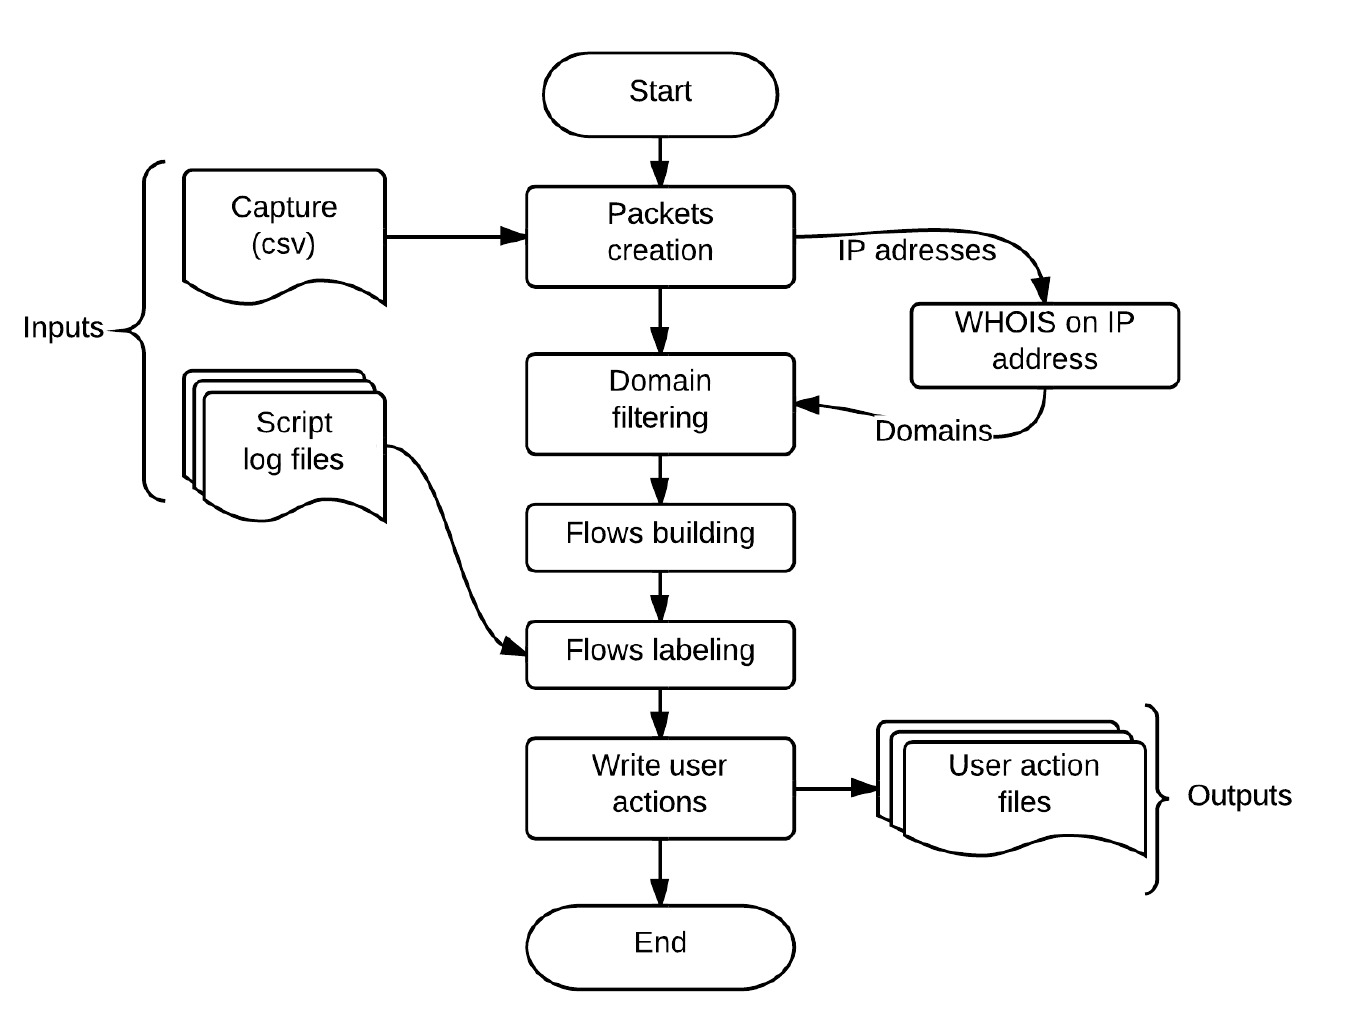
\includegraphics[width=300px]{method.jpeg}
    \end{center}
       \caption{network traffic pre-processing and labeling procedure}
    \label{fig:long}
    \label{fig:onecol}
    \end{figure}

    \begin{figure}[h]
    \begin{center}
       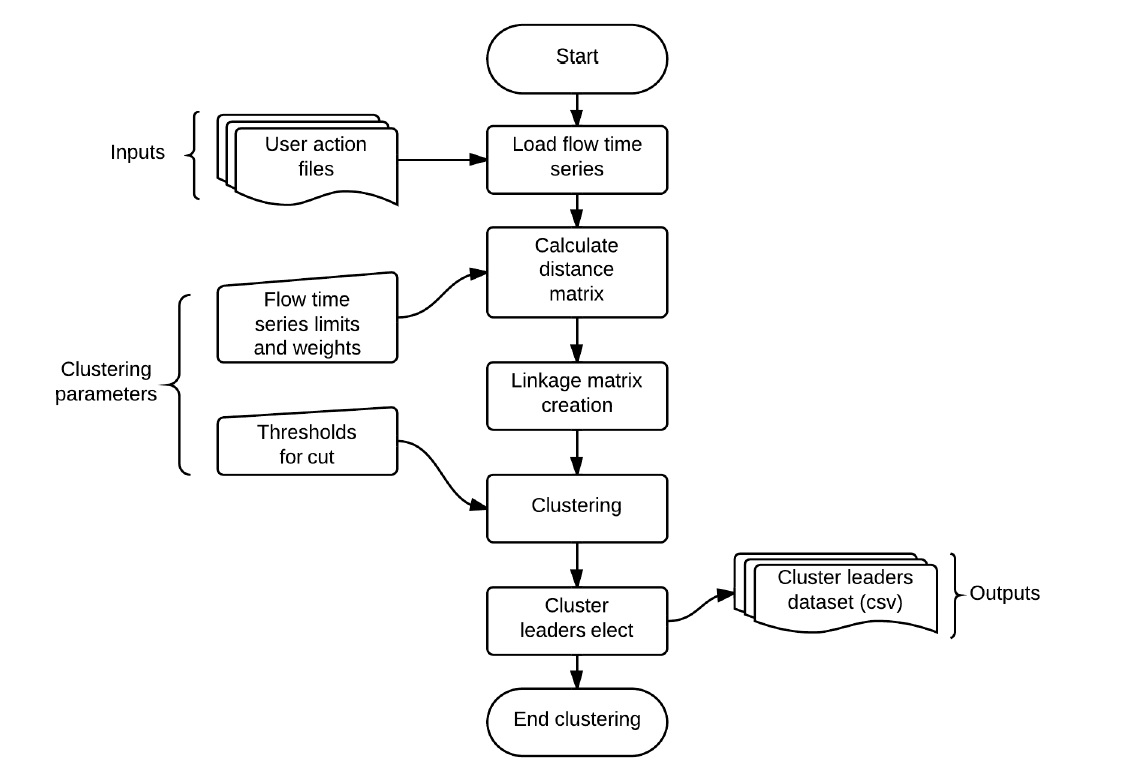
\includegraphics[width=300px]{cluster.jpg}
    \end{center}
       \caption{Flowchart for clustering procedure}
    \label{fig:long}
    \label{fig:onecol}
    \end{figure} 
    
\subsection{Network traffic pre-processing and labeling }
As a first step, we needed to create feature vectors out of the network traffic which was generated on using a particular mobile application. We used a MotoX with Android version 5.1 (Lollipop) to capture the network traffic generated by the Facebook mobile application. Using ADB shell commands, we emulated basic user interactions of touch ,type and swipe. Using these we simulated 20 iterations of three user interactions on Facebook:
\begin{itemize}
    \item Posting on a user wall
    \item Sending a message
    \item Open a user profile
\end{itemize}
Code for event generation is available in \textbf{data\_collection\_script.py}. 
We captured the packets generated by this through Wireshark. Using the Wireshark scripting functionality, we extracted each flow and created a separate pcap file for every flow [\textbf{extract\_flow.py}]. \\\\
We removed the packets responsible for ACKs, retransmissions, SYN, SYN-ACK, DNS and IGMP so that only the relevant packets are remaining [\textbf{filter\_flow.py}]. We also filtered out the flows based on IP which are related only to Facebook [\textbf{label\_flow.py}]. \\\\
We then labelled the flows in terms of the user actions by labelling all flows whose start time stamp or end time stamp was lying between the duration of event end plus 10 seconds [\textbf{label\_flow.py}].
As shown in Figure 3 then created a feature vector per flow comprising of three arrays containing packet sizes of the outgoing, ingoing and combined incoming and outgoing packets [\textbf{write\_feature.py}].

\begin{figure}[h]
    \begin{center}
       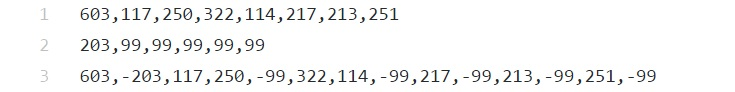
\includegraphics[width=400px]{feature.jpg}
    \end{center}
       \caption{A feature vector. The first array shows the packet size of the outgoing packets, the second for the incoming packets and the third for both. }
    \label{fig:long}
    \label{fig:onecol}
    \end{figure}

We are only considering packets which were transmitted upto 10 seconds after the user interaction was completed for a event (post on wall, send message etc.). Also we filtered out features which had length smaller than 8. At the end of this process, we obtained 93 feature vectors.

\subsection{Clustering}
For clustering, we needed a distance metric. We have used the dynamic time warping algorithm to align any two feature vectors. Specifically to find the distance between any two arrays containing packet lengths, we are using the \textbf{fast-dtw} python package. We then used \textbf{scipy.cluster.hierarchy} in SciPy python library [\textbf{clustering.py}]. We tried clustering the feature vectors with different weights assigned to each of the incoming, outgoing and incoming+outgoing feature vectors.\\\\
We were able to cluster the feature vectors with varying packet distributions for different weights. The following dendogram for instance, shows the packet distribution in which the weights for the outgoing distribution have been assigned as 1, and 0 for both the incoming and incoming+outgoing feature vectors. As the figure 4 shows the clusters are sufficiently separated.

    \begin{figure}[h]
    \begin{center}
       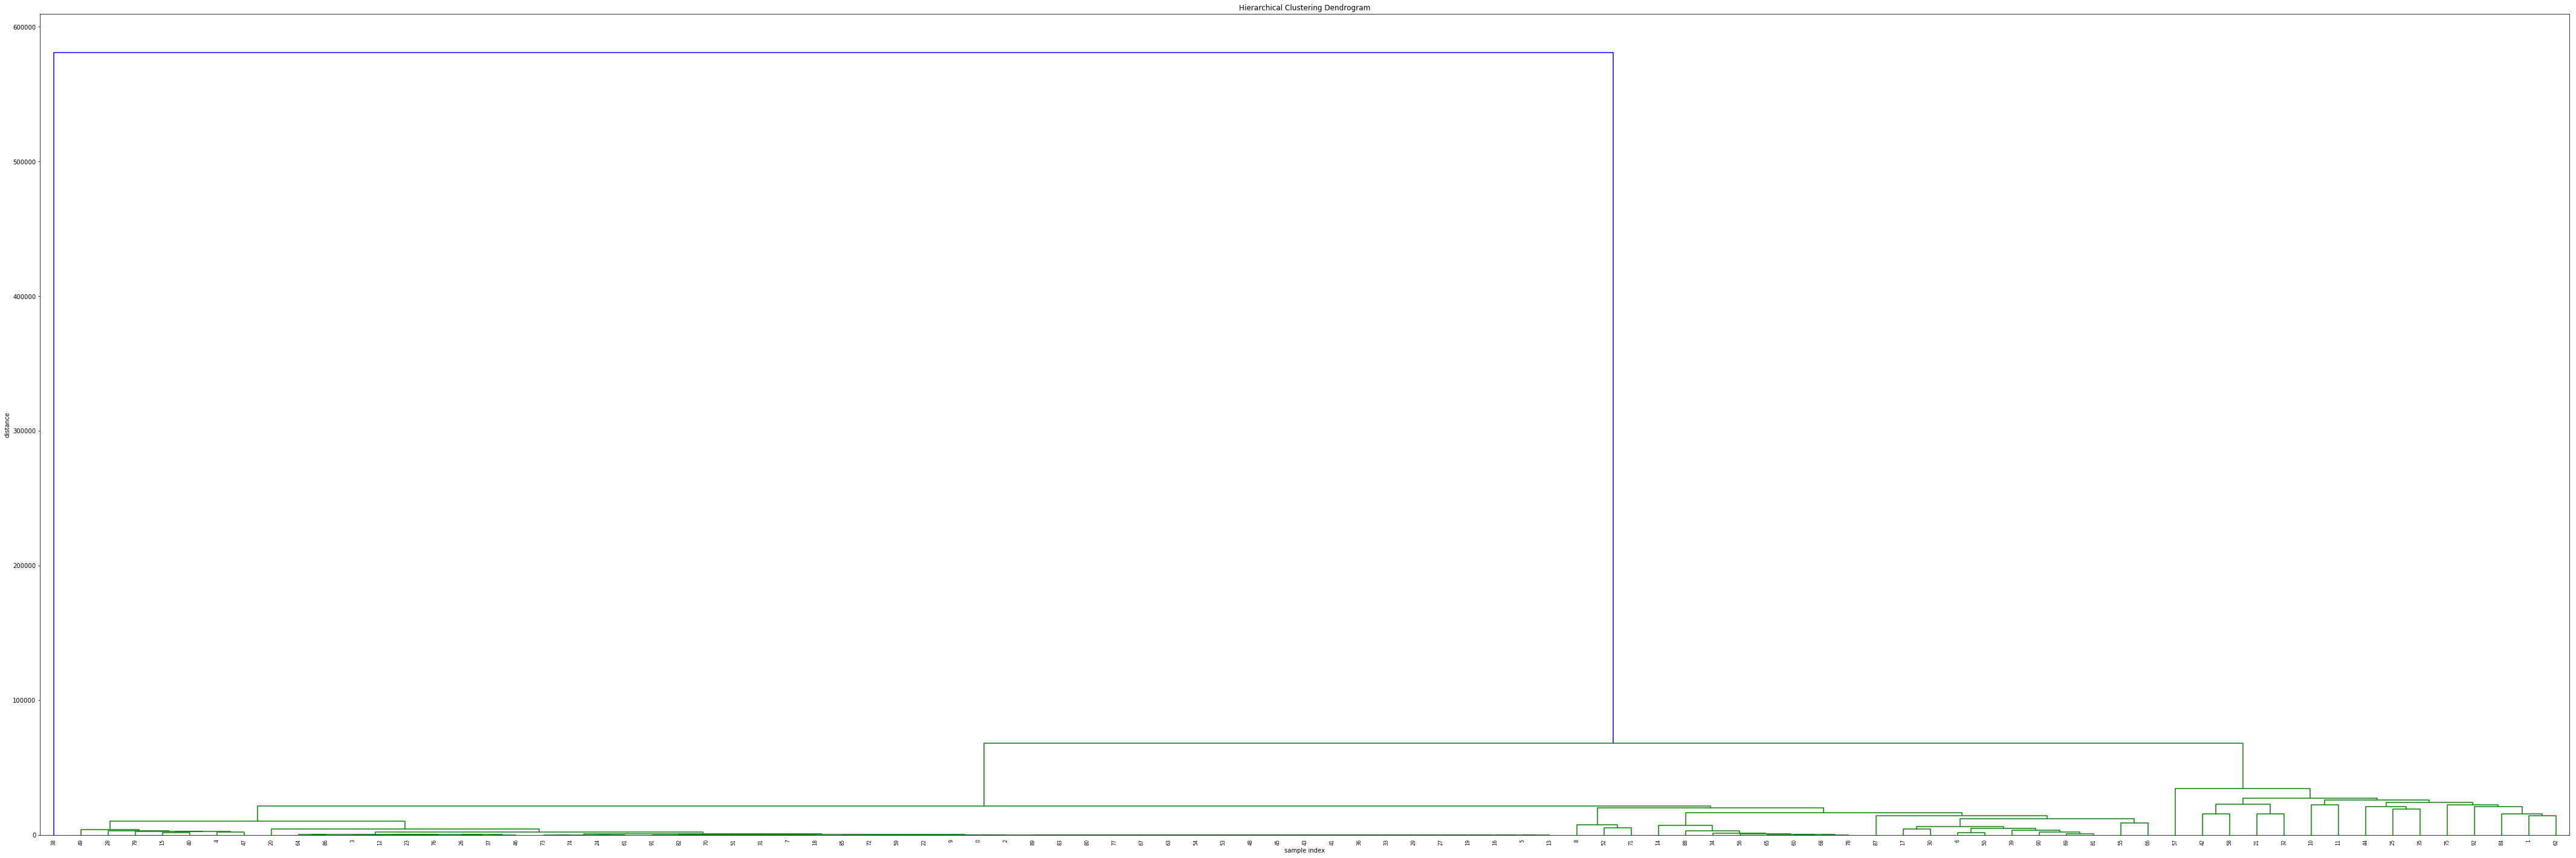
\includegraphics[width=400px]{dendogram_outweight_1.png}
    \end{center}
       \caption{Dendogram }
    \label{fig:long}
    \label{fig:onecol}
    \end{figure}
    
\section{Remaining work}
At present we have only considered unsupervised classification by using hierarchical clustering. It remains to see how the Precision, recall matrices perform using this approach. We also want to use a supervised classification approach. Finally we want to do this whole procedure for another application like gmail etc.

\section{References}
Can't you hear me knocking: Identification of user actions on Android apps via traffic analysis. \textit{Mauro Conti, Luigi V. Mancini, Riccardo Spolaor, Nino V. Verde}
\end{document}